\documentclass[]{article}
\usepackage{lmodern}
\usepackage{amssymb,amsmath}
\usepackage{ifxetex,ifluatex}
\usepackage{fixltx2e} % provides \textsubscript
\ifnum 0\ifxetex 1\fi\ifluatex 1\fi=0 % if pdftex
  \usepackage[T1]{fontenc}
  \usepackage[utf8]{inputenc}
\else % if luatex or xelatex
  \ifxetex
    \usepackage{mathspec}
  \else
    \usepackage{fontspec}
  \fi
  \defaultfontfeatures{Ligatures=TeX,Scale=MatchLowercase}
\fi
% use upquote if available, for straight quotes in verbatim environments
\IfFileExists{upquote.sty}{\usepackage{upquote}}{}
% use microtype if available
\IfFileExists{microtype.sty}{%
\usepackage{microtype}
\UseMicrotypeSet[protrusion]{basicmath} % disable protrusion for tt fonts
}{}
\usepackage[margin=1in]{geometry}
\usepackage{hyperref}
\hypersetup{unicode=true,
            pdftitle={Rintermediate: R and Probability distributions},
            pdfauthor={Mette Langaas, Martina Hall and Oyvind Bakke, Department of Mathematical Sciences, NTNU},
            pdfborder={0 0 0},
            breaklinks=true}
\urlstyle{same}  % don't use monospace font for urls
\usepackage{color}
\usepackage{fancyvrb}
\newcommand{\VerbBar}{|}
\newcommand{\VERB}{\Verb[commandchars=\\\{\}]}
\DefineVerbatimEnvironment{Highlighting}{Verbatim}{commandchars=\\\{\}}
% Add ',fontsize=\small' for more characters per line
\usepackage{framed}
\definecolor{shadecolor}{RGB}{248,248,248}
\newenvironment{Shaded}{\begin{snugshade}}{\end{snugshade}}
\newcommand{\KeywordTok}[1]{\textcolor[rgb]{0.13,0.29,0.53}{\textbf{#1}}}
\newcommand{\DataTypeTok}[1]{\textcolor[rgb]{0.13,0.29,0.53}{#1}}
\newcommand{\DecValTok}[1]{\textcolor[rgb]{0.00,0.00,0.81}{#1}}
\newcommand{\BaseNTok}[1]{\textcolor[rgb]{0.00,0.00,0.81}{#1}}
\newcommand{\FloatTok}[1]{\textcolor[rgb]{0.00,0.00,0.81}{#1}}
\newcommand{\ConstantTok}[1]{\textcolor[rgb]{0.00,0.00,0.00}{#1}}
\newcommand{\CharTok}[1]{\textcolor[rgb]{0.31,0.60,0.02}{#1}}
\newcommand{\SpecialCharTok}[1]{\textcolor[rgb]{0.00,0.00,0.00}{#1}}
\newcommand{\StringTok}[1]{\textcolor[rgb]{0.31,0.60,0.02}{#1}}
\newcommand{\VerbatimStringTok}[1]{\textcolor[rgb]{0.31,0.60,0.02}{#1}}
\newcommand{\SpecialStringTok}[1]{\textcolor[rgb]{0.31,0.60,0.02}{#1}}
\newcommand{\ImportTok}[1]{#1}
\newcommand{\CommentTok}[1]{\textcolor[rgb]{0.56,0.35,0.01}{\textit{#1}}}
\newcommand{\DocumentationTok}[1]{\textcolor[rgb]{0.56,0.35,0.01}{\textbf{\textit{#1}}}}
\newcommand{\AnnotationTok}[1]{\textcolor[rgb]{0.56,0.35,0.01}{\textbf{\textit{#1}}}}
\newcommand{\CommentVarTok}[1]{\textcolor[rgb]{0.56,0.35,0.01}{\textbf{\textit{#1}}}}
\newcommand{\OtherTok}[1]{\textcolor[rgb]{0.56,0.35,0.01}{#1}}
\newcommand{\FunctionTok}[1]{\textcolor[rgb]{0.00,0.00,0.00}{#1}}
\newcommand{\VariableTok}[1]{\textcolor[rgb]{0.00,0.00,0.00}{#1}}
\newcommand{\ControlFlowTok}[1]{\textcolor[rgb]{0.13,0.29,0.53}{\textbf{#1}}}
\newcommand{\OperatorTok}[1]{\textcolor[rgb]{0.81,0.36,0.00}{\textbf{#1}}}
\newcommand{\BuiltInTok}[1]{#1}
\newcommand{\ExtensionTok}[1]{#1}
\newcommand{\PreprocessorTok}[1]{\textcolor[rgb]{0.56,0.35,0.01}{\textit{#1}}}
\newcommand{\AttributeTok}[1]{\textcolor[rgb]{0.77,0.63,0.00}{#1}}
\newcommand{\RegionMarkerTok}[1]{#1}
\newcommand{\InformationTok}[1]{\textcolor[rgb]{0.56,0.35,0.01}{\textbf{\textit{#1}}}}
\newcommand{\WarningTok}[1]{\textcolor[rgb]{0.56,0.35,0.01}{\textbf{\textit{#1}}}}
\newcommand{\AlertTok}[1]{\textcolor[rgb]{0.94,0.16,0.16}{#1}}
\newcommand{\ErrorTok}[1]{\textcolor[rgb]{0.64,0.00,0.00}{\textbf{#1}}}
\newcommand{\NormalTok}[1]{#1}
\usepackage{longtable,booktabs}
\usepackage{graphicx,grffile}
\makeatletter
\def\maxwidth{\ifdim\Gin@nat@width>\linewidth\linewidth\else\Gin@nat@width\fi}
\def\maxheight{\ifdim\Gin@nat@height>\textheight\textheight\else\Gin@nat@height\fi}
\makeatother
% Scale images if necessary, so that they will not overflow the page
% margins by default, and it is still possible to overwrite the defaults
% using explicit options in \includegraphics[width, height, ...]{}
\setkeys{Gin}{width=\maxwidth,height=\maxheight,keepaspectratio}
\IfFileExists{parskip.sty}{%
\usepackage{parskip}
}{% else
\setlength{\parindent}{0pt}
\setlength{\parskip}{6pt plus 2pt minus 1pt}
}
\setlength{\emergencystretch}{3em}  % prevent overfull lines
\providecommand{\tightlist}{%
  \setlength{\itemsep}{0pt}\setlength{\parskip}{0pt}}
\setcounter{secnumdepth}{0}
% Redefines (sub)paragraphs to behave more like sections
\ifx\paragraph\undefined\else
\let\oldparagraph\paragraph
\renewcommand{\paragraph}[1]{\oldparagraph{#1}\mbox{}}
\fi
\ifx\subparagraph\undefined\else
\let\oldsubparagraph\subparagraph
\renewcommand{\subparagraph}[1]{\oldsubparagraph{#1}\mbox{}}
\fi

%%% Use protect on footnotes to avoid problems with footnotes in titles
\let\rmarkdownfootnote\footnote%
\def\footnote{\protect\rmarkdownfootnote}

%%% Change title format to be more compact
\usepackage{titling}

% Create subtitle command for use in maketitle
\newcommand{\subtitle}[1]{
  \posttitle{
    \begin{center}\large#1\end{center}
    }
}

\setlength{\droptitle}{-2em}

  \title{Rintermediate: R and Probability distributions}
    \pretitle{\vspace{\droptitle}\centering\huge}
  \posttitle{\par}
  \subtitle{TMA4268 Statistical Learning V2019. Module 1: INTRODUCTION TO
STATISTICAL LEARNING}
  \author{Mette Langaas, Martina Hall and Oyvind Bakke, Department of Mathematical
Sciences, NTNU}
    \preauthor{\centering\large\emph}
  \postauthor{\par}
      \predate{\centering\large\emph}
  \postdate{\par}
    \date{week 2, 2019}

\usepackage{xcolor}

\begin{document}
\maketitle

{
\setcounter{tocdepth}{2}
\tableofcontents
}
\definecolor{dg}{rgb}{0,.25,0}

(Latest changes: 31.12.18: first version for 2019)

Before working with this file you should have worked with the Rbeginner
file:
\url{https://www.math.ntnu.no/emner/TMA4268/2019v/1Intro/Rbeginner.html}

If you read the solutions version (file name ending in ``sol'') the
\textbf{solutions to \emph{exercises} are included.} (For the advanced
user: toggle solutions on/off in Rmd-file with variable
\texttt{showsol}.)

\begin{itemize}
\tightlist
\item
  Version without solutions:
  \url{https://www.math.ntnu.no/emner/TMA4268/2019v/1Intro/Rintermediate-sol.html}
\item
  Version with solutions:
  \url{https://www.math.ntnu.no/emner/TMA4268/2019v/1Intro/Rintermediate-sol.html}
\end{itemize}

(to see .Rmd or .pdf just replace in links above)

\section{Random variables and probability
distributions}\label{random-variables-and-probability-distributions}

To be able to do statistics, a good understanding of random variables
and probability distributions is vital.

\subsection{Background}\label{background}

Do you read Norwegian and want to brush up on these topics (theory, not
R)? Then go to the thematic pages from TMA4240/TMA4245 Statistics and
read about:

\begin{itemize}
\tightlist
\item
  \href{https://wiki.math.ntnu.no/tma4245/tema/begreper/variable}{Random
  variables and probability distributions}
\item
  \href{https://wiki.math.ntnu.no/tma4245/tema/begreper/discrete}{Important
  discrete distributions}
\item
  \href{https://wiki.math.ntnu.no/tma4245/tema/begreper/continuous}{Important
  continuous distributions}
\end{itemize}

We will also make a function to do a \(z\)-test (so, just a bit of
inference) and to calculate a \(p\)-value.

\section{Probability distributions in
R}\label{probability-distributions-in-r}

Tools for working with probability distributions are included in the
default environment in R, and we will now look at the \emph{binomial}
(discrete) distribution and the \emph{normal}, \emph{chi-squared},
\emph{t} and Fisher \emph{F} (continuous distribution). The multivariate
normal distribution will be covered in the interatice lecture of Module
2 of TMA4268 (and is also a large part of TMA4267).

For each of these distributions, there exists functions that calculates
the pdf (probability density or mass function, often denoted \(f\) in
previous courses), the cumulative distribution function (often denoted
\(F\)), the inverse cumulative distribution function (often denoted
\(F^{-1}\)) and drawing random numbers form the given distribution. For
the normal distribution these functions are called:

\begin{longtable}[]{@{}ll@{}}
\toprule
Function & Meaning\tabularnewline
\midrule
\endhead
dnorm & density (pdf)\tabularnewline
pnorm & cumulative distribution function (cdf)\tabularnewline
qnorm & inverse cumulative distribution (quantile
function)\tabularnewline
rnorm & draw random variable from normal distribution\tabularnewline
\bottomrule
\end{longtable}

NA

Remember to check the help pages of the functions you want to use, to
see what is used as input for each function. We will now look at each of
these functions.

\section{\texorpdfstring{Probability density or mass function
\(f(x)\)}{Probability density or mass function f(x)}}\label{probability-density-or-mass-function-fx}

\subsection{Binomial distibution}\label{binomial-distibution}

If we study a discrete distibution -- like the binomial distribution --
the probability mass function gives the probability of observing \(x\),
\(f(x) = P(X = x)\).

\textbf{Exercise:} What are the requirements that a random variable
\(X\) follows a binomial distribution? What are the parameters of the
distribution?

\begingroup\color{dg}

\endgroup

To plot the pdf of the binomial we may construct a barplot. We do this
now using the \texttt{ggplot2} package.

\begin{Shaded}
\begin{Highlighting}[]
\KeywordTok{library}\NormalTok{(ggplot2)}
\NormalTok{n =}\StringTok{ }\DecValTok{10}
\NormalTok{p =}\StringTok{ }\FloatTok{0.2}
\NormalTok{probs =}\StringTok{ }\KeywordTok{dbinom}\NormalTok{(}\DecValTok{0}\OperatorTok{:}\DecValTok{10}\NormalTok{, n, p)}
\NormalTok{df =}\StringTok{ }\KeywordTok{data.frame}\NormalTok{(}\DataTypeTok{x =} \DecValTok{0}\OperatorTok{:}\DecValTok{10}\NormalTok{, }\DataTypeTok{y =}\NormalTok{ probs)}
\NormalTok{p <-}\StringTok{ }\KeywordTok{ggplot}\NormalTok{(}\DataTypeTok{data =}\NormalTok{ df, }\KeywordTok{aes}\NormalTok{(}\DataTypeTok{x =}\NormalTok{ x, }\DataTypeTok{y =}\NormalTok{ y)) }\OperatorTok{+}\StringTok{ }\KeywordTok{geom_bar}\NormalTok{(}\DataTypeTok{stat =} \StringTok{"identity"}\NormalTok{) }\OperatorTok{+}\StringTok{ }
\StringTok{    }\KeywordTok{theme_minimal}\NormalTok{()}
\NormalTok{p}
\end{Highlighting}
\end{Shaded}

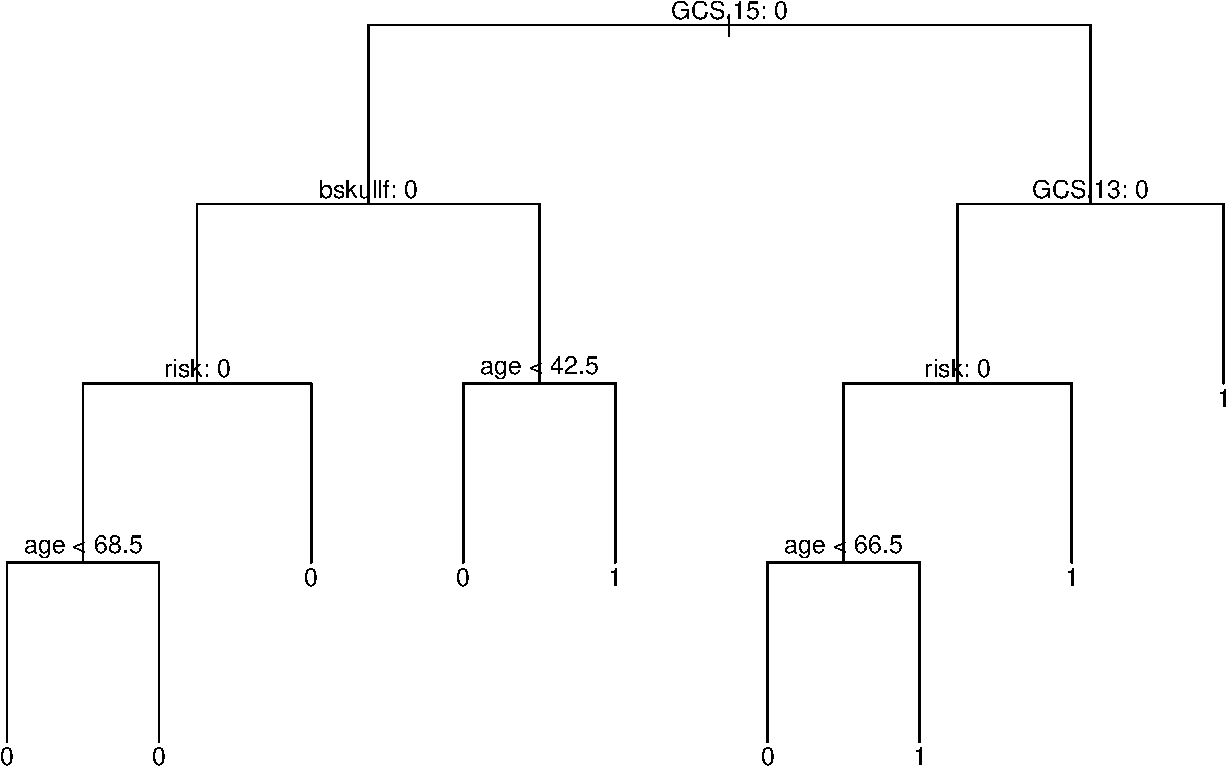
\includegraphics{Rintermediate_files/figure-latex/unnamed-chunk-2-1.pdf}

\textbf{Exercise:} Do the same, but with \(p=0.5\). Which value for
\(p\) do you think will be best if you need to approximate the binomial
with a normal distribution?

\begingroup\color{dg}

\endgroup

\subsection{Normal distribution}\label{normal-distribution}

For the continuous distributions -- like the normal distributions -- the
probability density function gives the probability of observing a value
between \(a\) and \(b\) when we integrate the pdf from \(a\) to \(b\):
\(P(a<X \le b)=\int_{a}^b f(x) dx\). Remember: \(f(x)\) does not give
the point probability of \(x\) - the point probability is 0. Why?

We can plot the pdf for the normal distribution:

\begin{Shaded}
\begin{Highlighting}[]
\NormalTok{x =}\StringTok{ }\KeywordTok{seq}\NormalTok{(}\DataTypeTok{from =} \OperatorTok{-}\DecValTok{5}\NormalTok{, }\DataTypeTok{to =} \DecValTok{5}\NormalTok{, }\DataTypeTok{length =} \DecValTok{100}\NormalTok{)}
\NormalTok{y =}\StringTok{ }\KeywordTok{dnorm}\NormalTok{(}\DataTypeTok{x =}\NormalTok{ x, }\DataTypeTok{mean =} \DecValTok{0}\NormalTok{, }\DataTypeTok{sd =} \DecValTok{1}\NormalTok{)}
\NormalTok{df =}\StringTok{ }\KeywordTok{data.frame}\NormalTok{(}\DataTypeTok{x =}\NormalTok{ x, }\DataTypeTok{y =}\NormalTok{ y)}
\NormalTok{p =}\StringTok{ }\KeywordTok{ggplot}\NormalTok{(}\DataTypeTok{data =}\NormalTok{ df, }\KeywordTok{aes}\NormalTok{(}\DataTypeTok{x =}\NormalTok{ x, }\DataTypeTok{y =}\NormalTok{ y)) }\OperatorTok{+}\StringTok{ }\KeywordTok{geom_line}\NormalTok{() }\OperatorTok{+}\StringTok{ }\KeywordTok{ggtitle}\NormalTok{(}\StringTok{"Standard normal pdf"}\NormalTok{) }\OperatorTok{+}\StringTok{ }
\StringTok{    }\KeywordTok{theme_minimal}\NormalTok{()}
\NormalTok{p}
\end{Highlighting}
\end{Shaded}

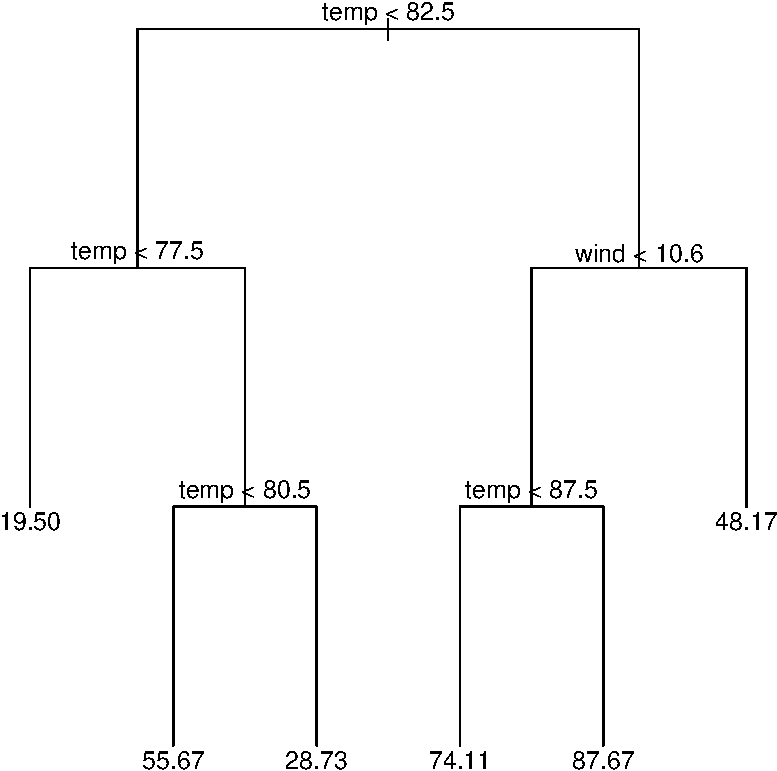
\includegraphics{Rintermediate_files/figure-latex/unnamed-chunk-4-1.pdf}

\textbf{Exercise:} Find \(f(1.4)\) looking at the figure \textbf{and}
using the \texttt{dnorm}. How can you interpret this value?

\begingroup\color{dg}

\endgroup

We can also plot the distribution using random generated values for the
distribution. The function \texttt{rnorm()} draws random values from the
given distribution. Below we draw \texttt{n=10000} values and make a
histogram.

\begin{Shaded}
\begin{Highlighting}[]
\NormalTok{n =}\StringTok{ }\DecValTok{10000}
\NormalTok{x =}\StringTok{ }\KeywordTok{rnorm}\NormalTok{(}\DataTypeTok{n =}\NormalTok{ n, }\DataTypeTok{mean =} \DecValTok{0}\NormalTok{, }\DataTypeTok{sd =} \DecValTok{1}\NormalTok{)}
\NormalTok{p =}\StringTok{ }\KeywordTok{ggplot}\NormalTok{(}\KeywordTok{data.frame}\NormalTok{(}\DataTypeTok{x =}\NormalTok{ x), }\KeywordTok{aes}\NormalTok{(x)) }\OperatorTok{+}\StringTok{ }\KeywordTok{geom_histogram}\NormalTok{() }\OperatorTok{+}\StringTok{ }\KeywordTok{theme_minimal}\NormalTok{()}
\NormalTok{p}
\end{Highlighting}
\end{Shaded}

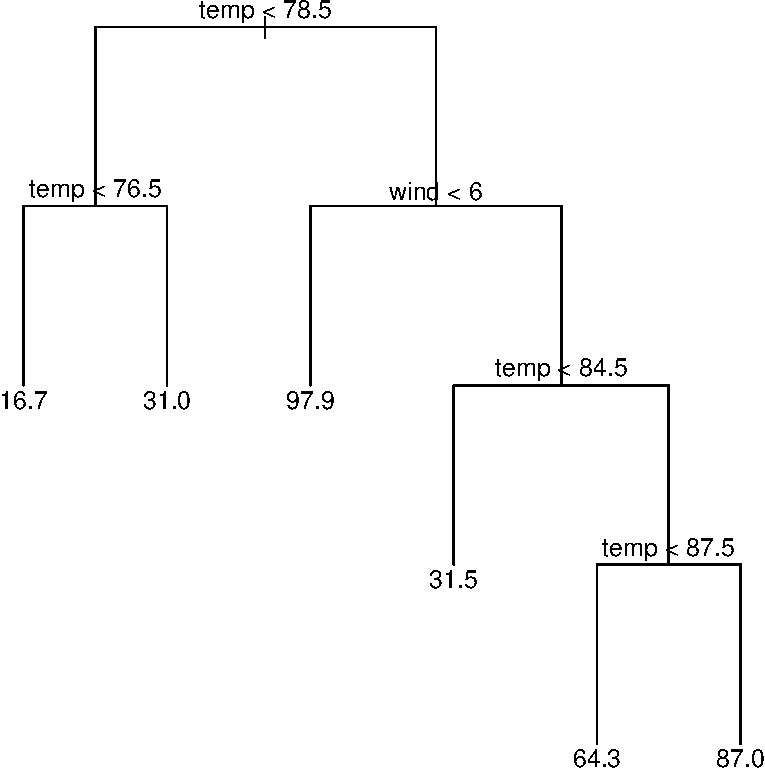
\includegraphics{Rintermediate_files/figure-latex/unnamed-chunk-6-1.pdf}

Try using smaller values of \texttt{n} and see what happends. Explain.

We can easily check the sample mean, variance and standard deviation of
our drawn values by

\begin{Shaded}
\begin{Highlighting}[]
\KeywordTok{mean}\NormalTok{(x)}
\KeywordTok{var}\NormalTok{(x)}
\KeywordTok{sd}\NormalTok{(x)}
\end{Highlighting}
\end{Shaded}

\textbf{Exercise:} Check your drawn values to see that the mean and
variance agree with what you specified. (No solution provided.)

\subsection{Chi-squared distribution}\label{chi-squared-distribution}

In our introductory course in statistics we learned that if \(X\) is a
standard normal variable then \(X^2\) is chi-squared distributed with
\(1\) degree of freedom.

\textbf{Exercise:} What is the expected value and variance of a
\(\chi^2\)-distribution with 1 degree of freedom? Look at the data drawn
from the standard normal distribution above, and calulate the sample
mean and variance of \texttt{x\^{}2}. Does your result coincide with the
known expected value and variance for this distribution? What happens to
your result if you increase or decrease \texttt{n}?

\begingroup\color{dg}

\endgroup

We may also draw values directly from the chi-squared distribution.

\begin{Shaded}
\begin{Highlighting}[]
\NormalTok{n =}\StringTok{ }\DecValTok{10000}
\NormalTok{x =}\StringTok{ }\KeywordTok{rchisq}\NormalTok{(}\DataTypeTok{n =}\NormalTok{ n, }\DataTypeTok{df =} \DecValTok{1}\NormalTok{)}
\NormalTok{p =}\StringTok{ }\KeywordTok{ggplot}\NormalTok{(}\KeywordTok{data.frame}\NormalTok{(}\DataTypeTok{x =}\NormalTok{ x), }\KeywordTok{aes}\NormalTok{(x)) }\OperatorTok{+}\StringTok{ }\KeywordTok{geom_histogram}\NormalTok{() }\OperatorTok{+}\StringTok{ }\KeywordTok{ggtitle}\NormalTok{(}\StringTok{"Chi^2 distribution"}\NormalTok{) }\OperatorTok{+}\StringTok{ }
\StringTok{    }\KeywordTok{theme_minimal}\NormalTok{()}
\NormalTok{p}
\end{Highlighting}
\end{Shaded}

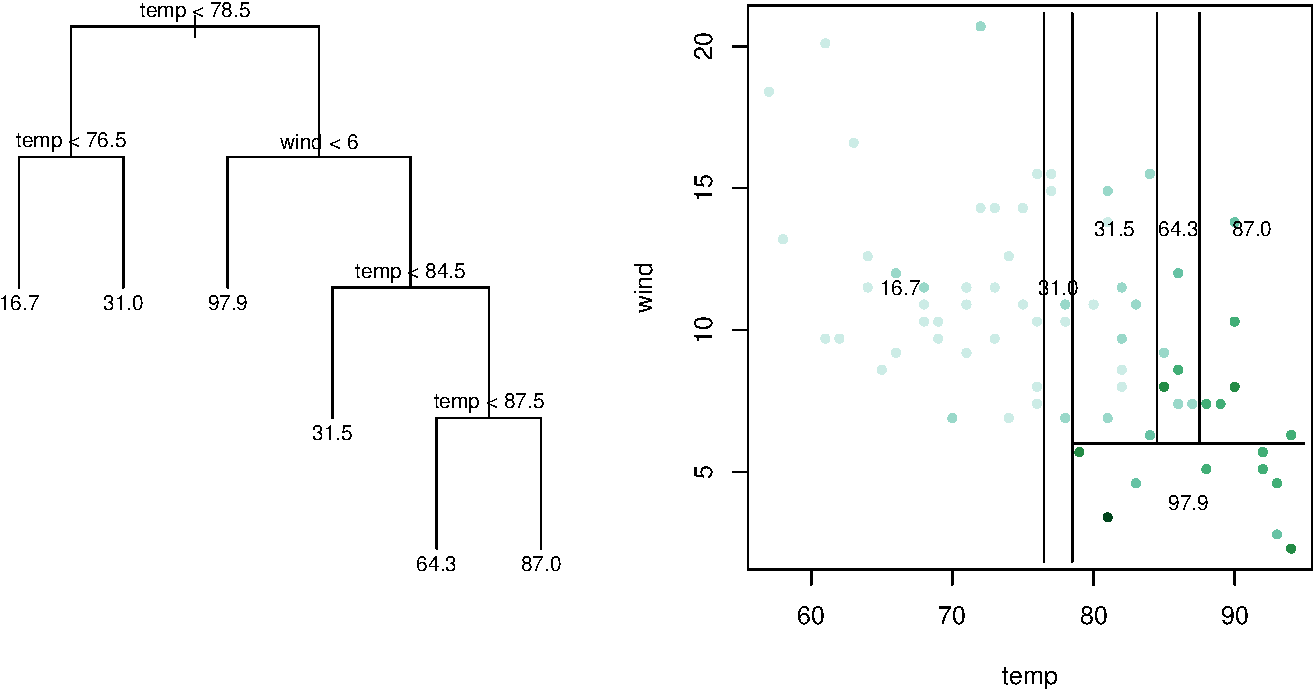
\includegraphics{Rintermediate_files/figure-latex/unnamed-chunk-9-1.pdf}

\subsection{t-distribution}\label{t-distribution}

Let \(X_i\) be independent normal variables with mean \(\mu\) and
variance \(\sigma^2\), and \(\bar{X}=\frac{1}{n}\sum_{i=1}^n X_i\) and
\(S^2=\frac{1}{n-1}\sum_{i=1}^n (X_i-\bar{X})^2\). Further let
\[ T=\frac{\bar{X}-\mu}{S/\sqrt{n}}\]

\textbf{Exercise:} What is the connection between \(S^2\) and the
chi-square distribution? What is the connection between \(T\) and the
\(t\)-distribution?

\begingroup\color{dg}

\endgroup

We can plot the pdf for the \(t\)-distribution with \(n-1\) degrees of
freedom, and add the standard normal for reference. Is the red curve the
\(t\) or normal curve? How can you see that?

\begin{Shaded}
\begin{Highlighting}[]
\KeywordTok{library}\NormalTok{(ggplot2)}
\NormalTok{n =}\StringTok{ }\DecValTok{10}
\NormalTok{x =}\StringTok{ }\KeywordTok{seq}\NormalTok{(}\DataTypeTok{from =} \OperatorTok{-}\DecValTok{5}\NormalTok{, }\DataTypeTok{to =} \DecValTok{5}\NormalTok{, }\DataTypeTok{length =} \DecValTok{100}\NormalTok{)}
\NormalTok{pdft =}\StringTok{ }\KeywordTok{dt}\NormalTok{(}\DataTypeTok{x =}\NormalTok{ x, }\DataTypeTok{df =}\NormalTok{ n }\OperatorTok{-}\StringTok{ }\DecValTok{1}\NormalTok{)}
\NormalTok{pdfn =}\StringTok{ }\KeywordTok{dnorm}\NormalTok{(x)}
\NormalTok{df =}\StringTok{ }\KeywordTok{data.frame}\NormalTok{(}\DataTypeTok{x =}\NormalTok{ x, }\DataTypeTok{pdft =}\NormalTok{ pdft, }\DataTypeTok{pdfn =}\NormalTok{ pdfn)}
\NormalTok{p =}\StringTok{ }\KeywordTok{ggplot}\NormalTok{(}\DataTypeTok{data =}\NormalTok{ df, }\KeywordTok{aes}\NormalTok{(}\DataTypeTok{x =}\NormalTok{ x)) }\OperatorTok{+}\StringTok{ }\KeywordTok{geom_line}\NormalTok{(}\KeywordTok{aes}\NormalTok{(}\DataTypeTok{x =}\NormalTok{ x, }\DataTypeTok{y =}\NormalTok{ pdft)) }\OperatorTok{+}\StringTok{ }
\StringTok{    }\KeywordTok{geom_line}\NormalTok{(}\KeywordTok{aes}\NormalTok{(}\DataTypeTok{x =}\NormalTok{ x, }\DataTypeTok{y =}\NormalTok{ pdfn), }\DataTypeTok{colour =} \StringTok{"red"}\NormalTok{) }\OperatorTok{+}\StringTok{ }\KeywordTok{theme_minimal}\NormalTok{()}
\NormalTok{p}
\end{Highlighting}
\end{Shaded}

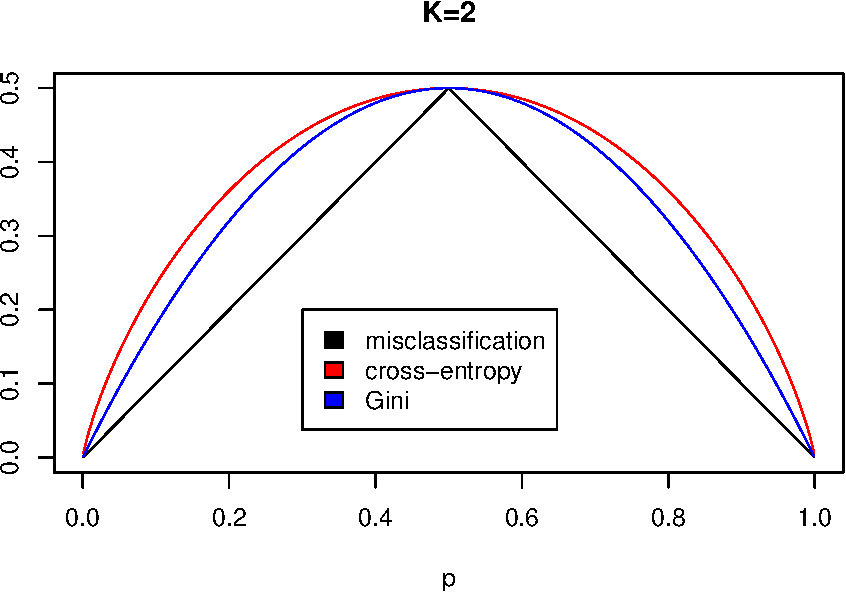
\includegraphics{Rintermediate_files/figure-latex/unnamed-chunk-11-1.pdf}

\subsection{The Fisher distribution}\label{the-fisher-distribution}

The final distribution is the Fisher distribution which is defined as a
ratio between scaled chi-squared random variables. Let
\(V\sim \chi^2(v)\) and \(W\sim \chi^2(w)\) then the ratio
\[\frac{V/v}{W/w}\sim F_{v,w}\] follows a Fisher distribution with \(v\)
and \(w\) degrees of freedom. We will use this distribution when working
with ratios of variance estimates.

\textbf{Exercise:} Plot the pdf for the Fisher distribution with \(v=5\)
and \(w=10\) degrees of freedom. Hint \texttt{df}.

\begingroup\color{dg}

\endgroup

\section{\texorpdfstring{Cumulative distribution function
\(F(x)\)}{Cumulative distribution function F(x)}}\label{cumulative-distribution-function-fx}

The cumulative distribution function (cdf) is the probability that your
observation is less or equal to x, \[F(x) = P(X\leq x) = 
\begin{cases} \int_{-\infty}^{x} f_x(t)dt \quad \text{for continuous distributions}\\
\sum_{t\leq x} f(t) \quad \text{for discrete distributions}
\end{cases}\]

The following plot shows the cdf of a standard normal distribution.

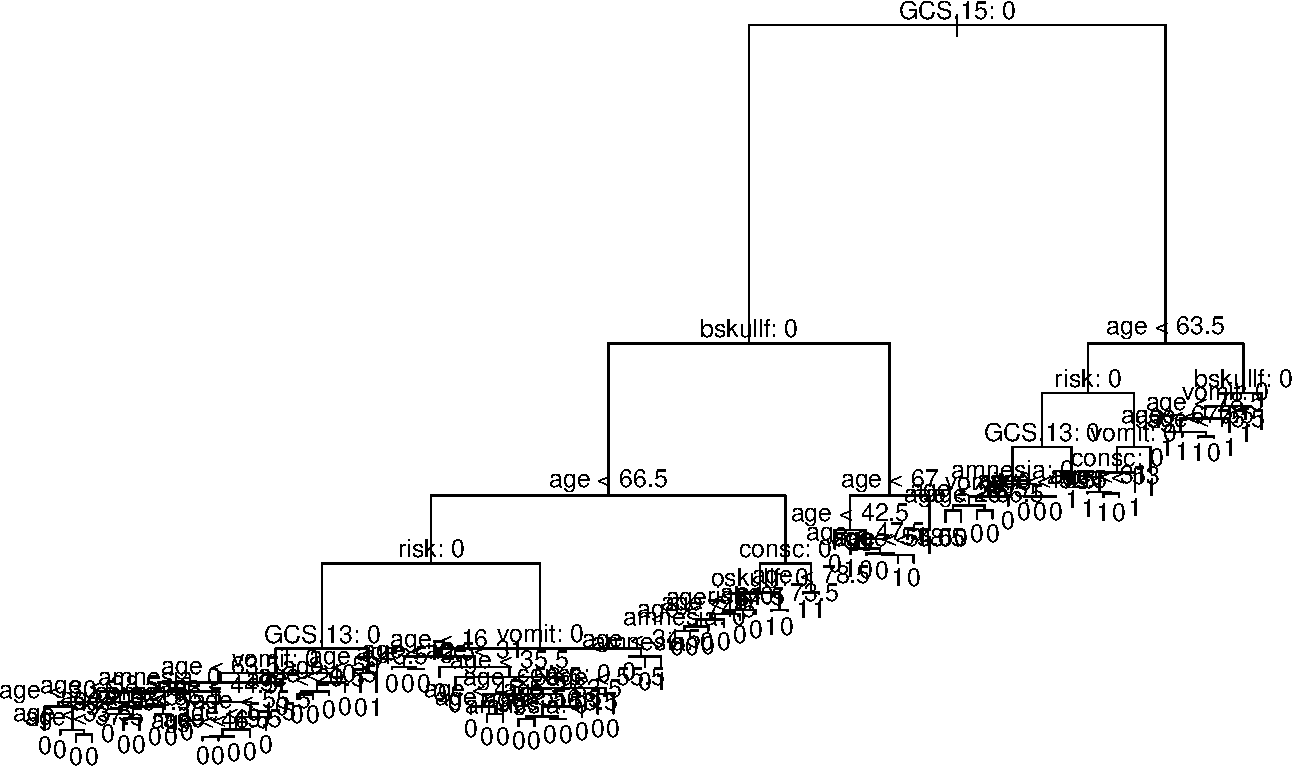
\includegraphics{Rintermediate_files/figure-latex/unnamed-chunk-14-1.pdf}

Below, we find the cdf of the critical values,
\(P(Z>z_{\alpha/2}) = \alpha/2\) and \(P(Z<z_{1-\alpha/2}) = \alpha/2\)
for a standard normal distribution. Instead of integrating, we can use
the distribution function \texttt{pnorm()}

\begin{Shaded}
\begin{Highlighting}[]
\NormalTok{x =}\StringTok{ }\KeywordTok{seq}\NormalTok{(}\DataTypeTok{from =} \OperatorTok{-}\DecValTok{5}\NormalTok{, }\DataTypeTok{to =} \DecValTok{5}\NormalTok{, }\DataTypeTok{length =} \DecValTok{100}\NormalTok{)}
\NormalTok{y =}\StringTok{ }\KeywordTok{dnorm}\NormalTok{(}\DataTypeTok{x =}\NormalTok{ x, }\DataTypeTok{mean =} \DecValTok{0}\NormalTok{, }\DataTypeTok{sd =} \DecValTok{1}\NormalTok{)}
\NormalTok{z =}\StringTok{ }\FloatTok{1.96}
\KeywordTok{qplot}\NormalTok{(x, y, }\DataTypeTok{geom =} \KeywordTok{c}\NormalTok{(}\StringTok{"point"}\NormalTok{, }\StringTok{"line"}\NormalTok{), }\DataTypeTok{main =} \StringTok{"Standard normal distribution"}\NormalTok{, }
    \DataTypeTok{xlab =} \StringTok{"x"}\NormalTok{, }\DataTypeTok{ylab =} \StringTok{"density(x)"}\NormalTok{) }\OperatorTok{+}\StringTok{ }\KeywordTok{geom_vline}\NormalTok{(}\DataTypeTok{xintercept =} \KeywordTok{c}\NormalTok{(}\OperatorTok{-}\NormalTok{z, }
\NormalTok{    z)) }\OperatorTok{+}\StringTok{ }\KeywordTok{theme_minimal}\NormalTok{()}
\end{Highlighting}
\end{Shaded}

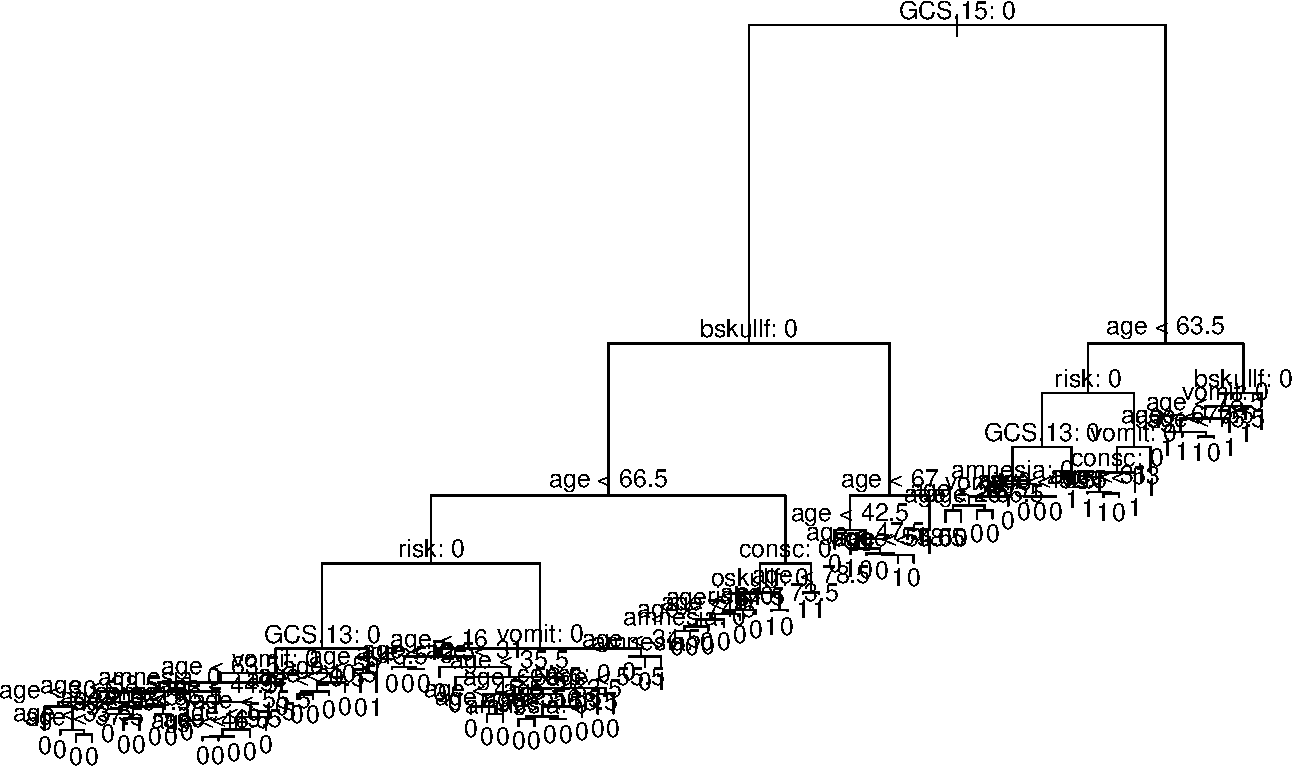
\includegraphics{Rintermediate_files/figure-latex/unnamed-chunk-15-1.pdf}

\begin{Shaded}
\begin{Highlighting}[]
\NormalTok{alpha_lower =}\StringTok{ }\KeywordTok{pnorm}\NormalTok{(}\DataTypeTok{q =} \OperatorTok{-}\NormalTok{z, }\DataTypeTok{mean =} \DecValTok{0}\NormalTok{, }\DataTypeTok{sd =} \DecValTok{1}\NormalTok{, }\DataTypeTok{lower.tail =} \OtherTok{TRUE}\NormalTok{)}
\NormalTok{alpha_upper =}\StringTok{ }\DecValTok{1} \OperatorTok{-}\StringTok{ }\KeywordTok{pnorm}\NormalTok{(}\DataTypeTok{q =}\NormalTok{ z, }\DataTypeTok{mean =} \DecValTok{0}\NormalTok{, }\DataTypeTok{sd =} \DecValTok{1}\NormalTok{, }\DataTypeTok{lower.tail =} \OtherTok{TRUE}\NormalTok{)}
\KeywordTok{c}\NormalTok{(alpha_lower, alpha_upper)}
\end{Highlighting}
\end{Shaded}

\begin{verbatim}
## [1] 0.0249979 0.0249979
\end{verbatim}

Note that for the upper tail, we could have written
\texttt{alpha\_upper\ =\ pnorm(q\ =\ q,\ mean\ =\ 0,\ sd\ =\ 1,\ lower.tail\ =\ FALSE)}.
The logical option \texttt{lower.tail} indicate if you want to calculate
the upper, \(P(X>x)\), or the lower, \(P(X\leq x)\), tail. The default
is \texttt{TRUE}, meaning that if you don't include this option as input
it will automatically calculate the lower tail.

\textbf{Exercise} Find the cdf of \(x=-5\) and \(x=5\) from looking at
the figure \textbf{and} using the distribution function in R.

\begingroup\color{dg}

\endgroup

Let's check that the critical values \(z_{\alpha/2}\) and
\(z_{1-\alpha/2}\) are -1.96 and 1.96 when \(\alpha = 0.05\). For this,
we use the quantile function (inverse cdf).

\begin{Shaded}
\begin{Highlighting}[]
\NormalTok{z_l =}\StringTok{ }\KeywordTok{qnorm}\NormalTok{(}\FloatTok{0.025}\NormalTok{, }\DataTypeTok{mean =} \DecValTok{0}\NormalTok{, }\DataTypeTok{sd =} \DecValTok{1}\NormalTok{)}
\NormalTok{z_u =}\StringTok{ }\KeywordTok{qnorm}\NormalTok{(}\FloatTok{0.975}\NormalTok{, }\DataTypeTok{mean =} \DecValTok{0}\NormalTok{, }\DataTypeTok{sd =} \DecValTok{1}\NormalTok{)}
\KeywordTok{c}\NormalTok{(z_l, z_u)}
\end{Highlighting}
\end{Shaded}

\begin{verbatim}
## [1] -1.959964  1.959964
\end{verbatim}

\textbf{Exercise} Assume a student t-distribution with 1 degree of
freedom, as in the figure below. Use the distribution function to

\begin{enumerate}
\def\labelenumi{\arabic{enumi}.}
\tightlist
\item
  Calculate the cdf of \(x=1.8\),
  \(F_x(1.8) = \int_{-\infty}^{1.8} f_x(x)dx\). 
\item
  Calculate \(P(0\leq x \leq 2)\).
\end{enumerate}

\begingroup\color{dg}

\endgroup

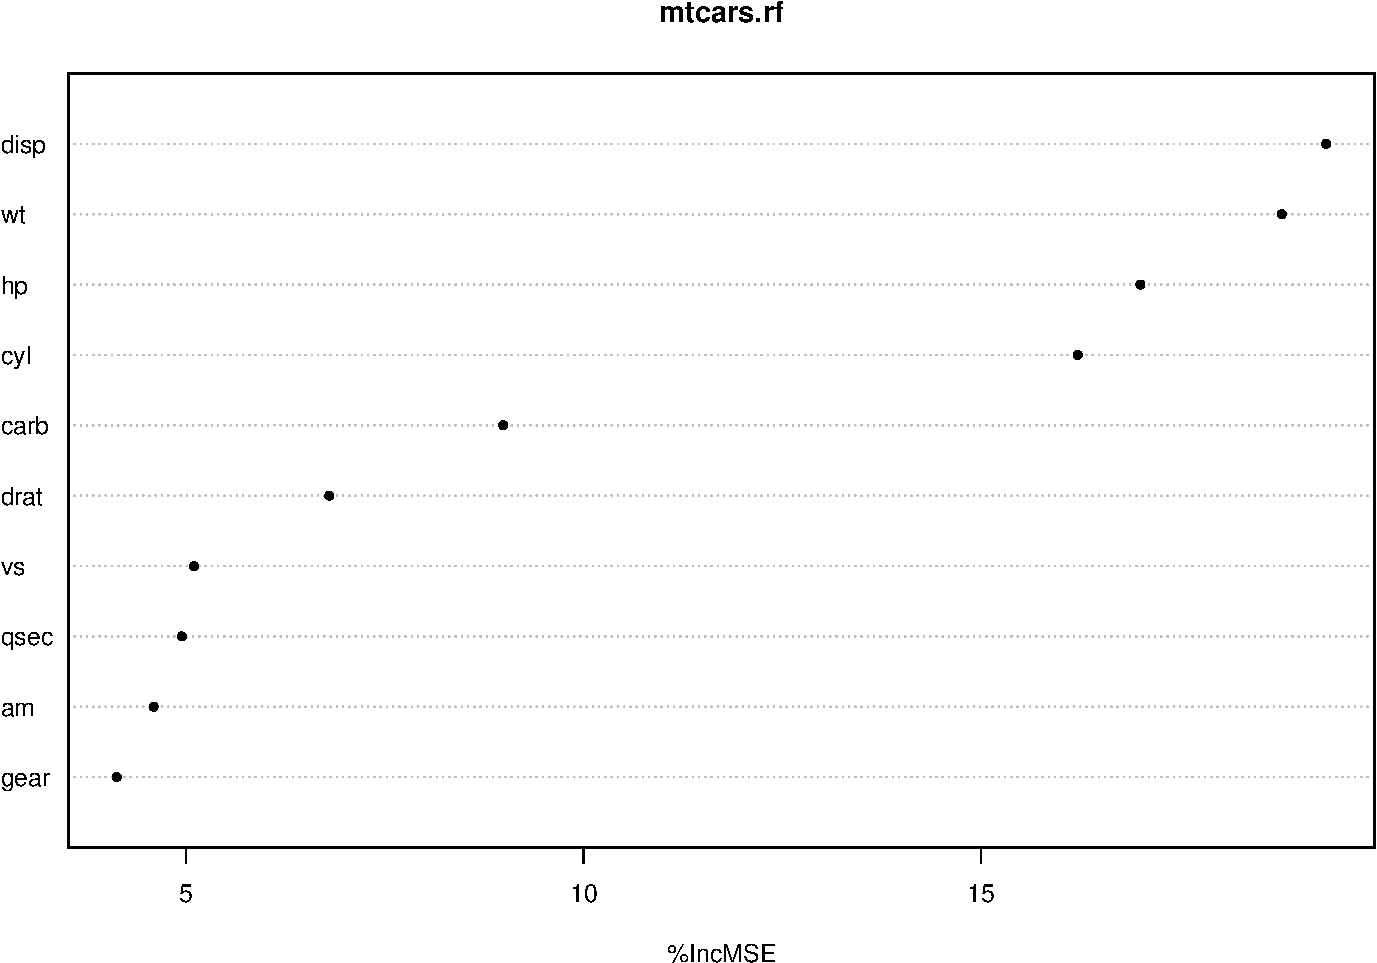
\includegraphics{Rintermediate_files/figure-latex/unnamed-chunk-20-1.pdf}

\section{Writing a simple Z-test as a
function}\label{writing-a-simple-z-test-as-a-function}

Let us assume that \(X\) is a random variable from a normal distribution
with know variance \(\sigma^2\) and we want to perform a hypothesis test
to test that the mean of \(X\) is not equal to \(0\), \(\mu\neq 0\),
that is, a two-sided test.

Assume that have collected a random sample \((X_1,X_2,\ldots,X_n)\), and
that we may assume that \(\frac{\bar{X}-\mu}{\sigma/\sqrt{n}}\) follows
a standard normal distribution (and \(\sigma^2\) is known). Here
\(\bar{X}=\frac{1}{n} \sum_{i=1}^n X_i\). A t-test is implemented in R
(function \texttt{t.test}) but no \texttt{z.test}, so now we (for the
sake of exercise) want to implement our own z-test.

Then we need a function with the data and given (known) standard
deviation as input. We assume that the data are given in a vector named
\texttt{x}.

Read and discuss what is done here.

\begin{Shaded}
\begin{Highlighting}[]
\NormalTok{myz.test <-}\StringTok{ }\ControlFlowTok{function}\NormalTok{(x, sd) \{}
\NormalTok{    n <-}\StringTok{ }\KeywordTok{length}\NormalTok{(x)}
\NormalTok{    xbar <-}\StringTok{ }\KeywordTok{mean}\NormalTok{(x)}
\NormalTok{    zobs <-}\StringTok{ }\NormalTok{xbar}\OperatorTok{/}\NormalTok{(sd}\OperatorTok{/}\KeywordTok{sqrt}\NormalTok{(n))}
    \CommentTok{# if you what to print remove hashtag in next line}
    \CommentTok{# print(paste('Zobs',zobs))}
\NormalTok{    pval <-}\StringTok{ }\DecValTok{2} \OperatorTok{*}\StringTok{ }\KeywordTok{pnorm}\NormalTok{(}\KeywordTok{abs}\NormalTok{(zobs), }\DataTypeTok{lower.tail =} \OtherTok{FALSE}\NormalTok{)}
    \CommentTok{# if you what to print remove hashtag in next line}
    \CommentTok{# print(paste('P-value',pval))}
    \KeywordTok{return}\NormalTok{(}\KeywordTok{list}\NormalTok{(}\DataTypeTok{statistic =}\NormalTok{ zobs, }\DataTypeTok{p.value =}\NormalTok{ pval))}
\NormalTok{\}}
\end{Highlighting}
\end{Shaded}

To use the function we first generate some data and then call the
function.

\begin{Shaded}
\begin{Highlighting}[]
\NormalTok{testds <-}\StringTok{ }\KeywordTok{rnorm}\NormalTok{(}\DecValTok{100}\NormalTok{, }\DataTypeTok{mean =} \FloatTok{0.5}\NormalTok{, }\DataTypeTok{sd =} \DecValTok{6}\NormalTok{)}
\KeywordTok{myz.test}\NormalTok{(testds, }\DataTypeTok{sd =} \DecValTok{6}\NormalTok{)}
\end{Highlighting}
\end{Shaded}

\begin{verbatim}
## $statistic
## [1] 1.012401
## 
## $p.value
## [1] 0.3113462
\end{verbatim}

If you want to run this function for many simulated data sets and put
the results from \texttt{myz.test} into a matrix you may use the
following simple for-loop:

\begin{Shaded}
\begin{Highlighting}[]
\NormalTok{mu =}\StringTok{ }\DecValTok{0}
\NormalTok{sigma =}\StringTok{ }\DecValTok{4}
\NormalTok{n =}\StringTok{ }\DecValTok{10}  \CommentTok{# size of each data set}
\NormalTok{B =}\StringTok{ }\DecValTok{1000}  \CommentTok{# number of data sets to simulate}
\NormalTok{results <-}\StringTok{ }\KeywordTok{matrix}\NormalTok{(}\OtherTok{NA}\NormalTok{, }\DataTypeTok{ncol =} \DecValTok{2}\NormalTok{, }\DataTypeTok{nrow =}\NormalTok{ B)}
\ControlFlowTok{for}\NormalTok{ (i }\ControlFlowTok{in} \DecValTok{1}\OperatorTok{:}\NormalTok{B) \{}
\NormalTok{    testX <-}\StringTok{ }\KeywordTok{rnorm}\NormalTok{(n, }\DataTypeTok{mean =}\NormalTok{ mu, }\DataTypeTok{sd =}\NormalTok{ sigma)}
\NormalTok{    thisresult <-}\StringTok{ }\KeywordTok{myz.test}\NormalTok{(testX, sigma)}
\NormalTok{    results[i, ] <-}\StringTok{ }\KeywordTok{c}\NormalTok{(thisresult}\OperatorTok{$}\NormalTok{statistic, thisresult}\OperatorTok{$}\NormalTok{p.value)}
\NormalTok{\}}
\KeywordTok{hist}\NormalTok{(results[, }\DecValTok{2}\NormalTok{])}
\end{Highlighting}
\end{Shaded}

\textbf{Exercise:} Run the code on your computer. What is done here?
What does the histogram display? Hint: what is the distribution of
\(p\)-values from true null hypotheses?

\begingroup\color{dg}

\endgroup

If you want reproducible results, it is useful to set the random
generator seed. That is done as \texttt{set.seed(a)} where \texttt{a} is
the seed you want to set.

\section{Plotting pdfs}\label{plotting-pdfs}

For the user who wants to do advanced graphics: Below is an example of
how to draw multiple plots using \texttt{ggplot}.

\textbf{Exercise:} What is this plot showing?

\begin{Shaded}
\begin{Highlighting}[]
\NormalTok{x =}\StringTok{ }\KeywordTok{seq}\NormalTok{(}\DataTypeTok{from =} \OperatorTok{-}\DecValTok{10}\NormalTok{, }\DataTypeTok{to =} \DecValTok{10}\NormalTok{, }\DataTypeTok{length =} \DecValTok{500}\NormalTok{)}
\NormalTok{y1 =}\StringTok{ }\KeywordTok{dnorm}\NormalTok{(x, }\DataTypeTok{mean =} \DecValTok{0}\NormalTok{, }\DataTypeTok{sd =} \DecValTok{1}\NormalTok{)}
\NormalTok{y2 =}\StringTok{ }\KeywordTok{dnorm}\NormalTok{(x, }\DataTypeTok{mean =} \DecValTok{0}\NormalTok{, }\DataTypeTok{sd =} \DecValTok{2}\NormalTok{)}
\NormalTok{y3 =}\StringTok{ }\KeywordTok{dnorm}\NormalTok{(x, }\DataTypeTok{mean =} \DecValTok{1}\NormalTok{, }\DataTypeTok{sd =} \DecValTok{2}\NormalTok{)}
\NormalTok{y4 =}\StringTok{ }\KeywordTok{dnorm}\NormalTok{(x, }\DataTypeTok{mean =} \OperatorTok{-}\DecValTok{1}\NormalTok{, }\DataTypeTok{sd =} \DecValTok{2}\NormalTok{)}
\NormalTok{df =}\StringTok{ }\KeywordTok{data.frame}\NormalTok{(x, y1, y2, y3, y4)}
\KeywordTok{ggplot}\NormalTok{(df, }\KeywordTok{aes}\NormalTok{(x, }\DataTypeTok{y =}\NormalTok{ value, }\DataTypeTok{color =}\NormalTok{ variable)) }\OperatorTok{+}\StringTok{ }\KeywordTok{geom_line}\NormalTok{(}\KeywordTok{aes}\NormalTok{(}\DataTypeTok{y =}\NormalTok{ y1, }
    \DataTypeTok{col =} \StringTok{"y1"}\NormalTok{)) }\OperatorTok{+}\StringTok{ }\KeywordTok{geom_line}\NormalTok{(}\KeywordTok{aes}\NormalTok{(}\DataTypeTok{y =}\NormalTok{ y2, }\DataTypeTok{col =} \StringTok{"y2"}\NormalTok{)) }\OperatorTok{+}\StringTok{ }\KeywordTok{geom_line}\NormalTok{(}\KeywordTok{aes}\NormalTok{(}\DataTypeTok{y =}\NormalTok{ y3, }
    \DataTypeTok{col =} \StringTok{"y3"}\NormalTok{)) }\OperatorTok{+}\StringTok{ }\KeywordTok{geom_line}\NormalTok{(}\KeywordTok{aes}\NormalTok{(}\DataTypeTok{y =}\NormalTok{ y4, }\DataTypeTok{col =} \StringTok{"y4"}\NormalTok{)) }\OperatorTok{+}\StringTok{ }\KeywordTok{ylim}\NormalTok{(}\DecValTok{0}\NormalTok{, }\FloatTok{0.5}\NormalTok{) }\OperatorTok{+}\StringTok{ }
\StringTok{    }\KeywordTok{ggtitle}\NormalTok{(}\StringTok{"Normal distribution"}\NormalTok{) }\OperatorTok{+}\StringTok{ }\KeywordTok{scale_colour_discrete}\NormalTok{(}\DataTypeTok{name =} \StringTok{"Mean, sd"}\NormalTok{, }
    \DataTypeTok{breaks =} \KeywordTok{c}\NormalTok{(}\StringTok{"y1"}\NormalTok{, }\StringTok{"y2"}\NormalTok{, }\StringTok{"y3"}\NormalTok{, }\StringTok{"y4"}\NormalTok{), }\DataTypeTok{labels =} \KeywordTok{c}\NormalTok{(}\StringTok{"0, 1"}\NormalTok{, }\StringTok{"0, 2"}\NormalTok{, }\StringTok{"1, 2 "}\NormalTok{, }
        \StringTok{"-1, 2"}\NormalTok{)) }\OperatorTok{+}\StringTok{ }\KeywordTok{theme_minimal}\NormalTok{()}
\end{Highlighting}
\end{Shaded}

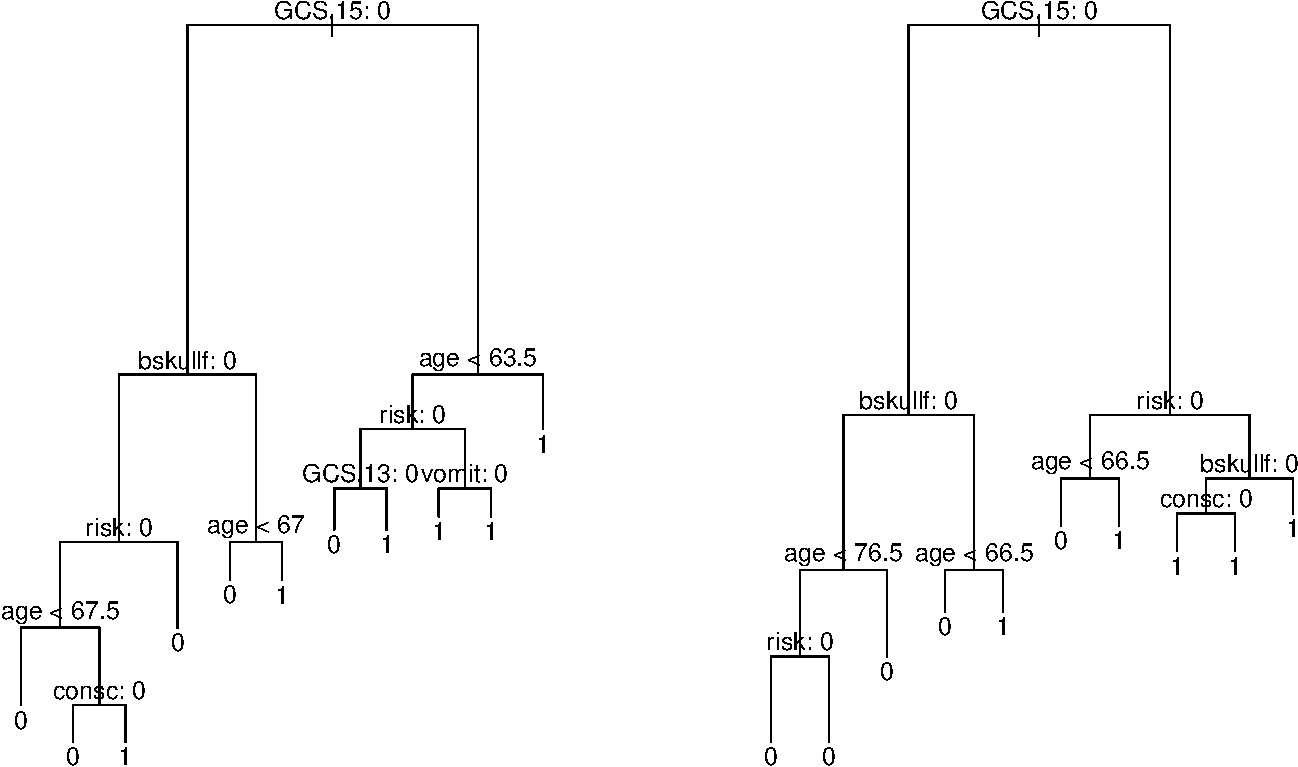
\includegraphics{Rintermediate_files/figure-latex/unnamed-chunk-25-1.pdf}

Let's assume we flip a coin where the probability of getting head is
\(p = P(head) = P(X=1) = 0.5\), and the probabiltiy of getting tails is
\(1-p = P(tails) = P(X=0)\). The following shows the number of times we
get head and tails of a throw when we try 1000 times

\begin{Shaded}
\begin{Highlighting}[]
\NormalTok{n =}\StringTok{ }\DecValTok{1000}
\NormalTok{p =}\StringTok{ }\FloatTok{0.5}
\NormalTok{x =}\StringTok{ }\KeywordTok{rbinom}\NormalTok{(n, }\DataTypeTok{size =} \DecValTok{1}\NormalTok{, }\DataTypeTok{prob =}\NormalTok{ p)}
\KeywordTok{qplot}\NormalTok{(x, }\DataTypeTok{geom =} \StringTok{"histogram"}\NormalTok{) }\OperatorTok{+}\StringTok{ }\KeywordTok{theme_minimal}\NormalTok{()}
\end{Highlighting}
\end{Shaded}

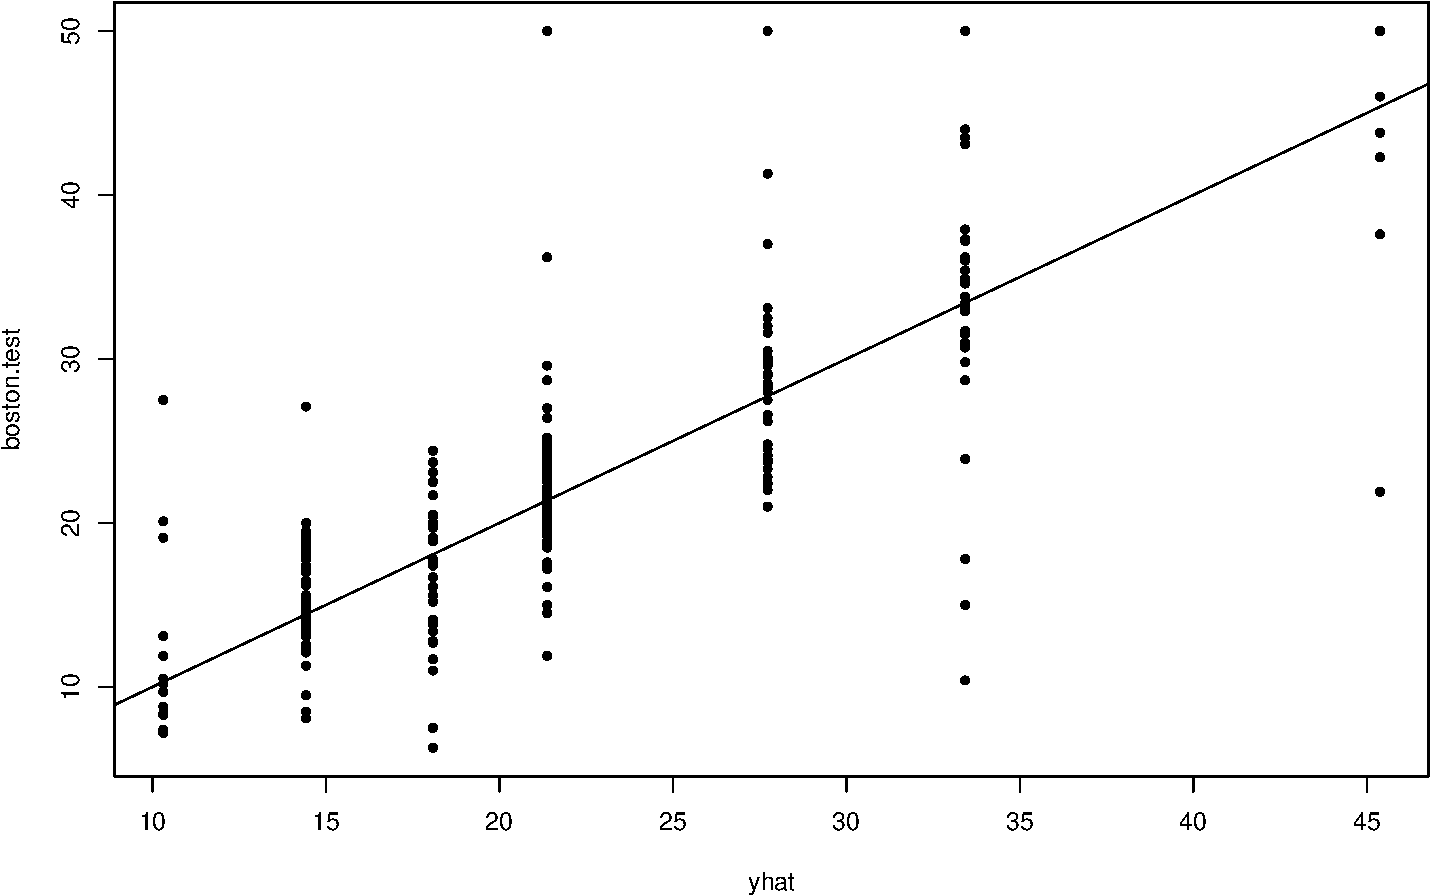
\includegraphics{Rintermediate_files/figure-latex/unnamed-chunk-26-1.pdf}

Note here that the option \texttt{size} refers the number of trials.

\textbf{Exercise:} Increase the number of trials to 100 when holding the
other parameters constant. Can you explain what happens here and why?
What is the mean and variance of this distribution? What is the
probability of having only one head when you do 100 trials?

\begingroup\color{dg}

\endgroup

\textbf{Exercise:} Make one plot of the pdf and one plot of the cdf for
each of the following distributions

\begin{enumerate}
\def\labelenumi{\arabic{enumi}.}
\tightlist
\item
  \(\chi^2\)- distributions with 1, 2, 3, 4, 6 and 9 degrees of freedom
\item
  Student t-distribution with 1, 2, 3, 4 and 5 degrees of freedom.
\end{enumerate}

\begingroup\color{dg}

\endgroup

Here is more about using \texttt{ggplot} to plot functions in general:
\url{http://t-redactyl.io/blog/2016/03/creating-plots-in-r-using-ggplot2-part-9-function-plots.html}


\end{document}
